\documentclass[letterpaper]{article}
\usepackage[submission]{aaai2027}
% The serif, sans-serif, and monospaced fonts are loaded automatically by aaai2027.sty.
\usepackage[hyphens]{url}
\usepackage{graphicx}
\urlstyle{rm}
\def\UrlFont{\rm}
\usepackage{natbib}
\usepackage{caption}
\frenchspacing
\usepackage{algorithm}
\usepackage{algorithmic}
\usepackage{amsmath,amssymb}
\usepackage{booktabs}
\pdfinfo{
/TemplateVersion (2027.1)
}
\setcounter{secnumdepth}{0}

\title{Reliability-Calibrated Mechanism Evidence Fusion}
\author{Anonymous Authors}
\affiliations{Anonymous Submission}

\begin{document}
\maketitle

\begin{abstract}
Industrial time-series fault diagnosis benefits from mechanism knowledge, yet industrial logs usually do not contain interventions. Control loops, delayed compensations, operating-condition shifts, and sparse fault labels make it unsafe to interpret every expert relation, statistical lag, or LLM-generated edge as a true causal effect. This paper studies a reliability-calibrated alternative. We treat expert rules, LLM condition-verifier outputs, lagged relations, residual dynamics, and graph paths as candidate mechanism evidence rather than recovered causal truth. A strong anchor discriminator remains the default predictor, and each mechanism source acts as a challenger that can modify the anchor only after validation-benefit, low-tail safety, counterfactual sensitivity, and source/complexity checks. The resulting Evidence Reliability Estimator learns when a candidate source is locally useful enough to correct the anchor. Across TEP, SKAB, Hydraulic, and C-MAPSS, the current evidence shows that reliability-calibrated mechanism admission improves or safely preserves strong models, with the strongest positive result on strict 22-class TEP fault diagnosis.
\end{abstract}

\section{Introduction}

Industrial time-series fault diagnosis is a natural testbed for knowledge-aware machine learning. Process variables are coupled by material flows, feedback control, delayed compensation, and regime-dependent operating states. A valve fault may first perturb a local flow, then propagate to pressure, temperature, or downstream quality variables after several time lags. These dynamics make purely pointwise diagnosis insufficient: a reliable model must reason over temporal evolution and process structure, while still maintaining strong predictive accuracy.

Existing diagnostic models expose a fundamental tension. Data-driven discriminators, including tree ensembles, temporal convolutional networks, recurrent models, Transformers, and graph-temporal networks, can learn powerful decision boundaries from historical logs. However, they mainly exploit observed statistical regularities, which may include spurious correlations induced by controllers, operating regimes, or label imbalance. Mechanism-aware approaches, such as expert graphs, process knowledge bases, and graph neural networks, provide useful structural priors, but industrial knowledge is often incomplete, static, and regime dependent. Large language models further expand this space by proposing fault mechanisms, key variables, lag ranges, signs, and weak-class rules, yet these proposals can be plausible without being predictive on the actual plant data.

The main difficulty is that real industrial logs are usually non-interventional. Operators rarely perturb valves, flows, temperatures, or pressures solely to identify causal effects, and safety constraints often make such interventions impossible. Consequently, it is unsafe to treat correlations, expert relations, statistical lags, or LLM-generated edges as a recovered true causal graph. This paper therefore studies a more practical and falsifiable question: when multiple unreliable sources provide candidate mechanism evidence, how can a model decide which evidence is reliable enough to correct a strong diagnostic predictor without causing negative transfer?

We formulate this as reliability-calibrated mechanism evidence admission for non-interventional industrial time-series diagnosis. A strong anchor discriminator remains the default predictor. Expert relations, LLM suggestions, lagged statistical relations, residual dynamics, and graph paths are treated as candidate challengers rather than authoritative causes. A challenger can influence the anchor only after passing validation-benefit, low-tail safety, counterfactual sensitivity, source trust, and complexity checks. The admitted evidence enters through constrained residual correction or weak-class verification rather than unchecked global logit editing.

The contributions are:
\begin{itemize}
  \item We reframe mechanism fusion in observational industrial logs as falsifiable candidate evidence admission rather than causal graph discovery.
  \item We introduce an Evidence Reliability Estimator that learns when an expert, LLM, statistical-lag, residual, or graph-path challenger is locally useful enough to correct a strong anchor.
  \item We design hierarchical edge admission: expert, LLM-assisted, and data-driven candidates are probed by source family, target group, lag group, and finally single edge before deployment.
  \item We implement residual/path-gated mechanism intervention so graph evidence can enter as an edge mask, attention bias, channel-fusion gate, or path relation only after reliability admission.
  \item We convert the LLM from an independent edge generator into an expert-graph conditional verifier whose outputs are conditional gate features until data support and validation admission approve them.
  \item We validate the framework through main comparisons, reliability ablations, mechanism ablations, and protocol audits across TEP, SKAB, Hydraulic, and C-MAPSS.
\end{itemize}

\section{Related Work}

\paragraph{Industrial time-series fault diagnosis.}
Classical process-monitoring, fault-diagnosis, and prognostics studies use process variables, temporal windows, and class-specific signatures to identify abnormal states or estimate remaining useful life. Benchmarks such as the Tennessee Eastman process \cite{downs1993tep}, SKAB \cite{skab2020}, Hydraulic \cite{helwig2018hydraulic}, and C-MAPSS \cite{saxena2008cmapss} expose multi-class process faults, run-level anomaly detection, component-state diagnosis, and RUL degradation modeling. Recent models use temporal encoders, reconstruction objectives, Transformers, or strong tabular discriminators to improve prediction. These methods can be effective anchors, but they usually optimize predictive accuracy directly and leave process mechanism evidence either implicit or post-hoc.

\paragraph{Graph and temporal dependency modeling.}
Graph-based time-series methods encode sensor relations, learned adjacency, or attention over variable interactions. Representative anomaly-detection families include graph-deviation and graph-attention approaches \cite{gdn2021,mtadgat2020}, Transformer and patch backbones such as TranAD, Anomaly Transformer, and PatchTST \cite{tranad2022,anomalytransformer2022,patchtst2023}, and graph-temporal forecasting models such as Graph WaveNet \cite{graphwavenet2019}. These approaches motivate the use of structure, but learned adjacency, attention weight, or edge gate is not equivalent to a deployment-safe mechanism claim. A relation can reduce training loss while still being unstable across regimes or harmful for low-tail groups.

\paragraph{LLM-assisted mechanism generation.}
Large language models can generate candidate fault mechanisms, important variables, lag ranges, sign constraints, propagation orders, and confusable counterexamples. This ability is useful for weak classes where labeled data are sparse and expert libraries are incomplete. However, LLM outputs are not measurements and should not be used as direct logit edits or authoritative causal edges. In our framework, the LLM acts conservatively as an expert-graph conditional verifier: it judges whether an expert edge or path should be active under a class, regime, residual state, or temporal pattern, and its output remains a gate feature until data support and reliability admission approve it.

\section{Problem Setup}

For a window or sample $i$, let $x_i$ be the multivariate industrial time-series input, $y_i$ the fault or state label, $r_i$ the residual evidence from normal dynamics, $g_i$ the operating or group context, and $m_k$ the $k$-th candidate mechanism item. A candidate may be an expert edge, an LLM condition-verifier feature for an expert edge or path, a lagged statistical relation, a residual-triggered graph path, or a source-pruned multi-edge structure.

The anchor prediction and candidate challenger predictions are:
\begin{equation}
\begin{aligned}
p_0(i) &= f_0(x_i),\\
p_k(i) &= f_k(x_i, r_i, g_i, m_k),\quad k=1,\ldots,K.
\end{aligned}
\end{equation}

$p_0$ is the default deployed prediction. $p_k$ is a mechanism-conditioned challenger. The problem is to learn when, if ever, $p_k$ should be allowed to modify the anchor. This setup makes the connection between the main classifier and later mechanism layers explicit: mechanism evidence is neither a disconnected explanation nor an unchecked post-processing module.

The anchor is the strong default predictor. A candidate mechanism evidence item is an expert rule, LLM proposal, lagged relation, residual signal, or graph path that may explain or improve a diagnostic decision. A challenger is the prediction route $p_k$ induced by one candidate evidence source. Reliability admission is the global certificate deciding whether a candidate may be deployed at all, and the Evidence Reliability Estimator is the local router estimating whether an admitted challenger should correct the anchor for sample $i$.

\begin{figure*}[t]
  \centering
  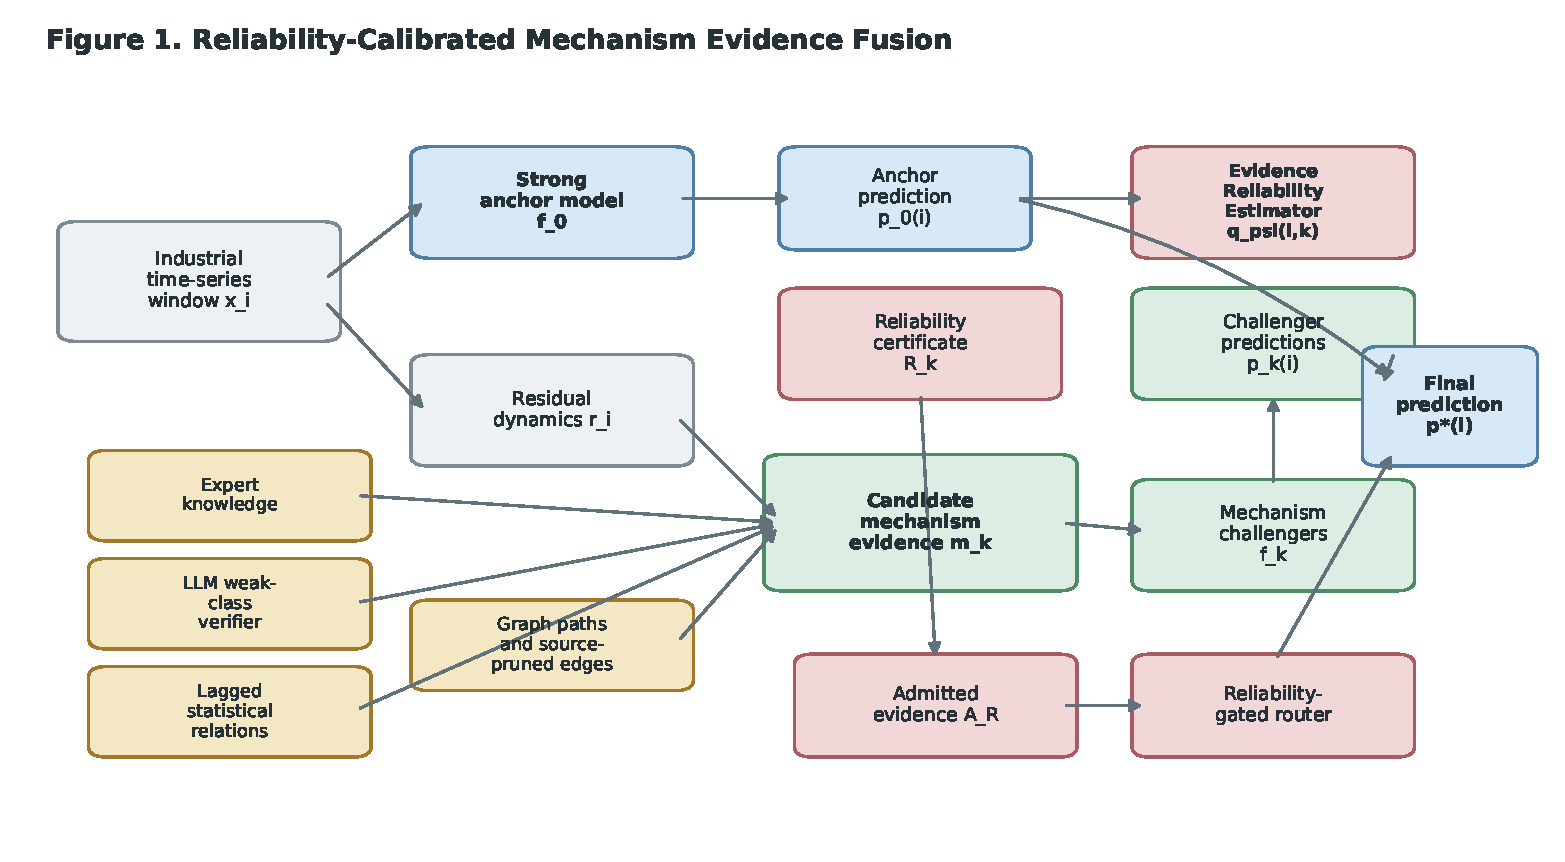
\includegraphics[width=0.95\textwidth]{figures/figure1_reliability_calibrated_mechanism_fusion.pdf}
  \caption{Reliability-calibrated mechanism evidence fusion. A strong anchor model remains the default predictor. Expert knowledge, LLM conditional verification, lagged statistics, residual dynamics, and graph paths generate candidate mechanism evidence. Evidence can modify the final prediction only if it passes the reliability certificate and local routing.}
  \label{fig:overview}
\end{figure*}

\section{Method}

\subsection{Anchor-Challenger Formulation}

The anchor model $f_0$ can be a TCN, GRU, Transformer, FT-Transformer, LightGBM, or another strong discriminator selected by the data protocol. The mechanism module does not replace this anchor by default. Instead, each mechanism evidence source creates a challenger. This formulation makes the fusion problem explicit: the question is not whether an auxiliary mechanism is plausible, but whether it is locally useful enough to improve the anchor under validation constraints.

For each candidate $m_k$, we define a local usefulness label:
\begin{equation}
z_{i,k} =
\mathbb{1}\left[
\ell(y_i,p_k(i)) + \delta < \ell(y_i,p_0(i))
\right],
\end{equation}
where $\ell$ is the task loss and $\delta$ is a margin preventing negligible changes from being labeled useful. The Evidence Reliability Estimator predicts:
\begin{equation}
q_{\psi}(i,k) =
\Pr(z_{i,k}=1 \mid x_i, r_i, g_i, \phi(m_k), p_0(i), p_k(i)).
\end{equation}

\subsection{Candidate Mechanism Evidence}

Candidate evidence comes from four sources. Expert evidence contributes process-flow relations, known equipment links, and sign constraints. Statistical evidence contributes lagged variable relations and residual changes under the declared split. LLM evidence no longer contributes independent final edges; it verifies whether expert edges or paths are conditionally active for a class, regime, residual state, or temporal pattern. Graph evidence composes these sources into paths, but the paths are treated as challengers rather than final explanations.

We do not inject a mixed edge pool as a whole. The candidate pool is frozen with source-family tags and then probed hierarchically: expert-only, LLM-only, and data-only source families are tested first; target-group and lag-group probes identify coarse harmful regions; single-edge probes then decide which relations can enter the deployment graph. This prevents a useful edge from being rejected merely because unrelated weak edges were tested in the same pool. Once an edge is admitted, its relation can enter as an edge mask, attention bias, channel-fusion gate, patch/frequency relation mask, or residual channel. The shifted target-minus-source channel used in some graph-temporal probes is therefore only one interface, not the definition of the method.

\subsection{Reliability Certificate}

Each candidate source receives a reliability certificate:
\begin{equation}
R_k =
\sigma(
\alpha_1 G_k -
\alpha_2 H_k +
\alpha_3 C_k +
\alpha_4 S_k -
\alpha_5 B_k),
\end{equation}
where $G_k$ is validation gain over the anchor, $H_k$ is low-tail harm, $C_k$ is counterfactual sensitivity, $S_k$ is source trust, and $B_k$ is complexity burden. The guards are ordered: $G_k$ and low-tail/FAR/MAR safety must pass before $C_k$ is evaluated. Counterfactual sensitivity verifies whether a model route depends on an admitted edge; it does not prove that the edge is useful. The admitted set is:
\begin{equation}
\mathcal{A}_R = \{k \mid R_k \ge \tau_R,\; G_k \ge 0,\; H_k \le \epsilon_H \}.
\end{equation}

This certificate is not an attention weight, edge gate, or static pruning score. It is a deployment admission criterion tied to observable validation benefit, harm control, and perturbation evidence.

\subsection{Reproducible Admission Algorithm}

Algorithm 1 gives the complete validation-only admission rule used by the paper package. First train the anchor $f_0$ and every challenger $f_k$ on the training split. Then freeze the candidate set and evaluate hierarchical probes on the validation split: source-family probes, target-group probes, lag-group probes, and finally single-edge probes. For each candidate, compute $G_k,H_k,C_k,S_k,B_k$, but in a fixed order: validation gain and low-tail/FAR/MAR safety are computed first, and counterfactual sensitivity is computed only after those guards pass. The remaining certificate terms $S_k$ and $B_k$ control source trust and complexity burden. All certificate terms use the same min--max normalization operator within the validation candidate pool, and no test labels are used to select candidates or thresholds. We grid-search only on validation:
\begin{equation}
\begin{aligned}
\mathcal{T}_R &= \{0.55,0.60,0.65,0.70\},\\
\tau_q &\in \{0.50,0.60,0.70\}.
\end{aligned}
\end{equation}
The selected result is a frozen deployment tuple $(f_0,\mathcal{A}_R,q_{\psi},\tau_R,\tau_q,\lambda_{\max})$. At test time this tuple is loaded without re-estimating thresholds, pruning edges, or changing source weights.

\subsection{Difference from Attention, Gates, and Pruning}

The proposed reliability step is not an ordinary gate inserted inside a neural network. An ordinary gate learns a differentiable importance multiplier during training, while our validation-only gate is an external admission decision that can reject a whole evidence source even if the source looks useful inside the training objective. It is also not an attention gate: attention redistributes representation mass among tokens, variables, or neighbors, whereas complete reliability admission decides whether a candidate mechanism can affect deployment at all. It differs from selective prediction because the system still returns a diagnostic or RUL output rather than abstaining. It differs from calibration because calibration changes confidence after a model is trained, whereas deployment risk control decides whether a mechanism challenger is allowed to override the anchor. Finally, it differs from pruning because the certificate combines validation gain, low-tail safety, counterfactual dependence, source trust, and complexity rather than keeping edges only by magnitude or sparsity.

\subsection{Deployment Rule}

At inference time, only admitted candidates can compete with the anchor:
\begin{equation}
k^*(i) =
\arg\max_{k \in \mathcal{A}_R} q_{\psi}(i,k).
\end{equation}
The final prediction is:
\begin{equation}
p^*(i) =
\begin{cases}
(1-\lambda_i)p_0(i)+\lambda_i p_{k^*}(i), & \text{if } q_{\psi}(i,k^*)\ge \tau_q,\\
p_0(i), & \text{otherwise},
\end{cases}
\end{equation}
where $\lambda_i$ is bounded by the reliability score. The anchor therefore remains the fallback whenever evidence is not admitted or locally unconvincing.

\begin{figure}[t]
  \centering
  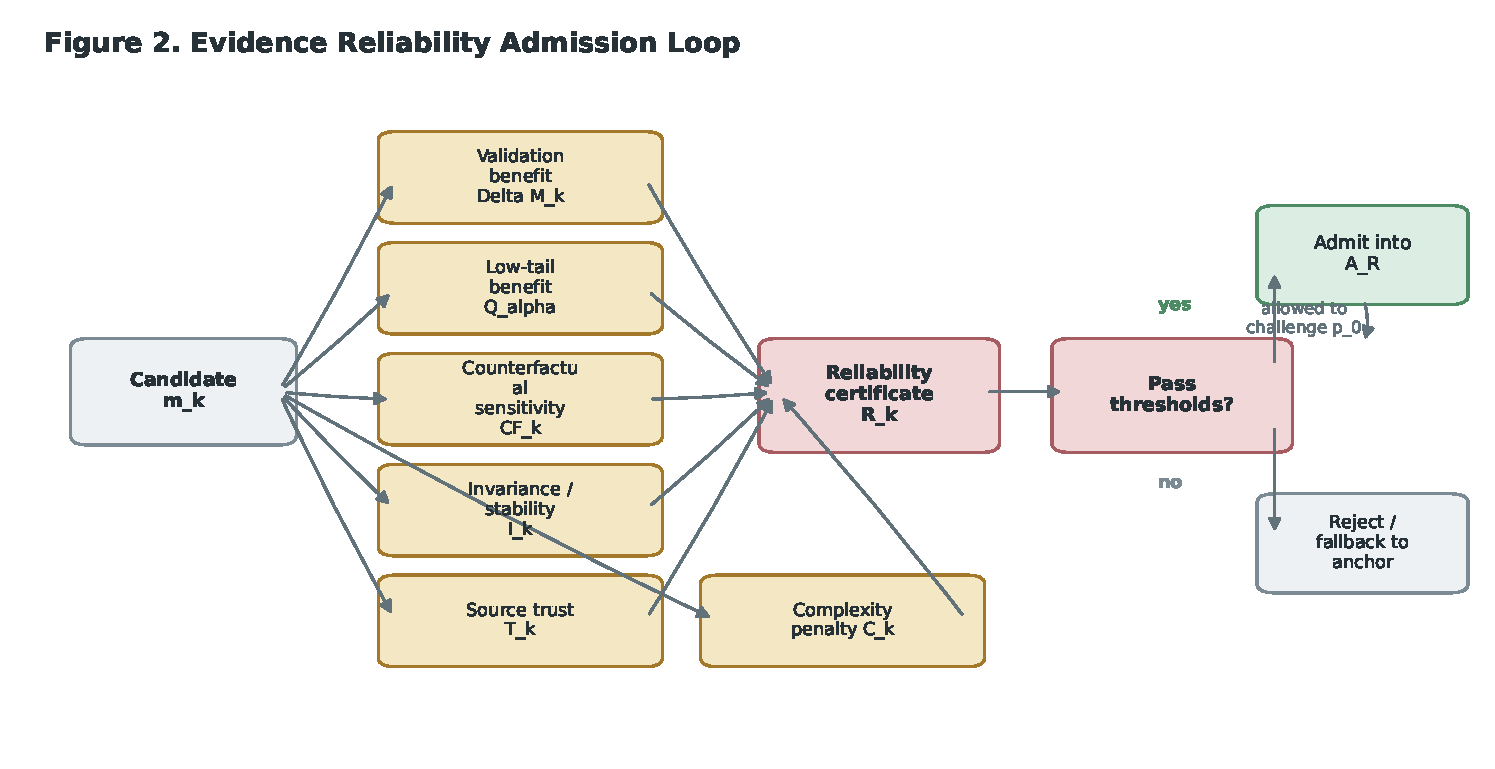
\includegraphics[width=0.98\linewidth]{figures/figure2_evidence_reliability_admission_loop.pdf}
  \caption{Evidence reliability admission loop. Mechanism evidence is proposed, converted into challengers, tested for validation gain, low-tail harm, counterfactual sensitivity, source trust, and complexity, then admitted or rejected.}
  \label{fig:ere-loop}
\end{figure}

\begin{figure}[t]
  \centering
  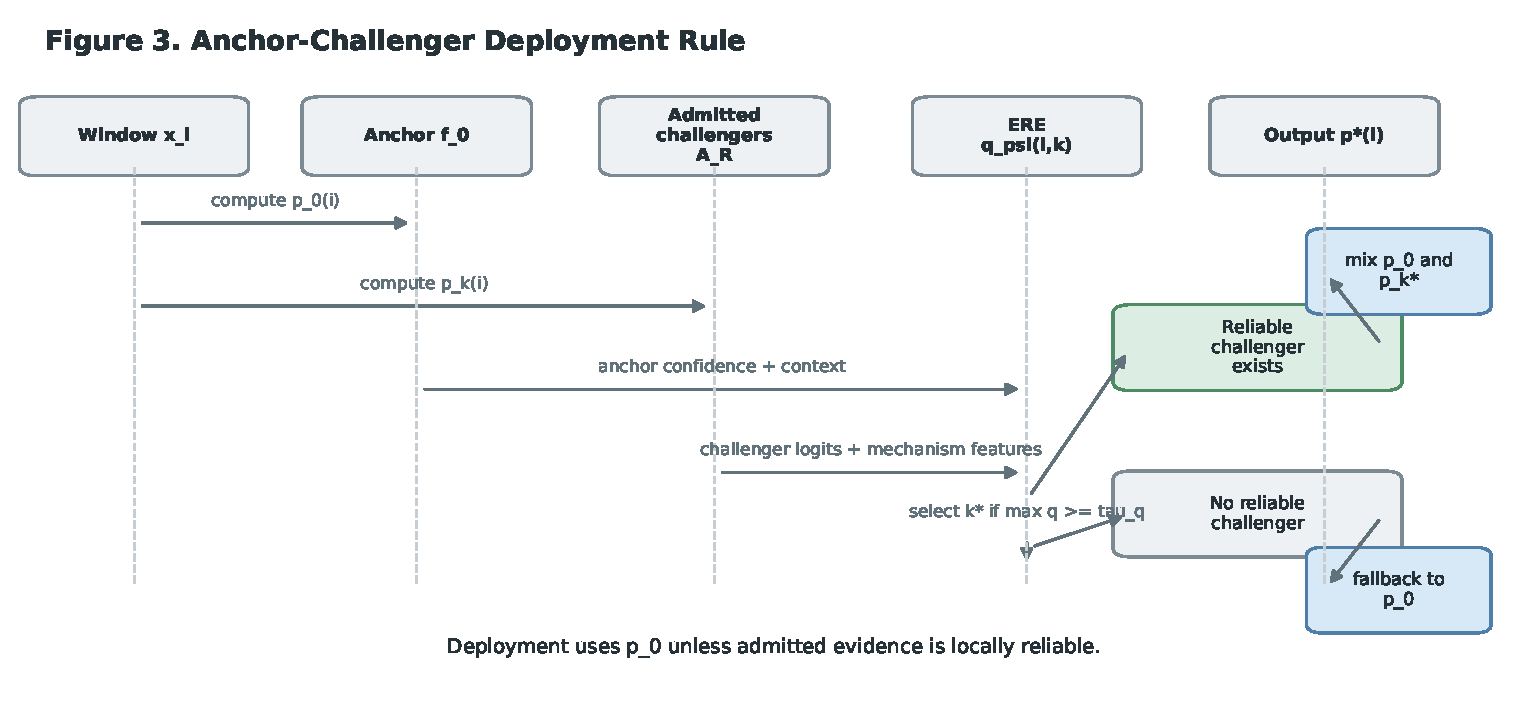
\includegraphics[width=0.98\linewidth]{figures/figure3_anchor_challenger_deployment_rule.pdf}
  \caption{Anchor-challenger deployment rule. The strong anchor is retained by default. A mechanism challenger can modify the decision only when the global certificate and local ERE score both pass thresholds.}
  \label{fig:deployment}
\end{figure}

\section{Theory and Claim Boundary}

This framework deliberately avoids claiming that observational logs identify the true causal graph. Instead, it makes a weaker and testable claim: under a fixed protocol, admitted candidate mechanism evidence should improve or preserve the anchor more often than unfiltered evidence. The optimization objective combines anchor learning, challenger learning, ERE calibration, and safety regularization:
\begin{equation}
\mathcal{L} =
\mathcal{L}_{0}
+ \beta_c \mathcal{L}_{c}
+ \beta_r \mathcal{L}_{ERE}
+ \beta_s \mathcal{L}_{safe}.
\end{equation}
The ERE term is supervised by local improvement labels, while the safety term penalizes low-tail harm and over-complex evidence admission. Counterfactual perturbation does not prove true causality; it verifies whether the model's decision uses the proposed mechanism route in the expected direction. This is a reliability test for model dependence, not a claim of physical intervention.

Disallowed claim before additional evidence: the method should not be described as recovering the plant's true causal graph or as proving universal benchmark superiority until matched external protocols, raw seed-level artifacts, and intervention-level evidence are available.

\section{Experiments}

\subsection{Experimental Questions}

The experiments are organized around four questions. RQ1 asks whether the full framework improves strong anchors under matched protocols. RQ2 asks whether reliability admission prevents harmful knowledge injection. RQ3 asks which mechanism sources contribute to performance. RQ4 asks whether the method preserves near-ceiling performance or transfer safety on auxiliary datasets.

\subsection{Datasets and Protocols}

TEP is the primary 22-class mechanism-diagnosis benchmark. SKAB evaluates binary anomaly detection and dynamic graph evidence in valve-related industrial time series. Hydraulic evaluates four component-state targets with near-ceiling baselines. C-MAPSS evaluates original terminal RUL regression and transfer across operating settings. We report strong matched-protocol evidence under stated protocols, not universal official SOTA claims, unless the split, preprocessing, metrics, thresholding, scoring rule, and training budget are exactly aligned with an external benchmark.

Split and leakage control are fixed before model selection: training data fit anchors and challengers, validation data select reliability thresholds and admitted candidates, and test data are used once for reporting. Window / label construction follows the dataset task rather than a single artificial target: TEP and SKAB use time-series windows for diagnosis or anomaly labels, Hydraulic uses component-state labels, and C-MAPSS uses terminal test-unit RUL. Metric and thresholding are likewise task-specific but validation-only: macro/target F1 for diagnosis or anomaly detection and RMSE/MAE/score for RUL. Seeds / budget are recorded for each formal run so that model families are compared under matched training limits. No test-set threshold or route tuning is allowed after the frozen deployment tuple is selected. Same reliability equation across datasets means that evidence admission remains comparable even when the anchor architecture changes. For C-MAPSS, a train-unit pseudo-terminal validation audit independently selects the same w160/cap150 temporal anchor by RMSE; it also discloses that PHM score has a secondary trade-off, so C-MAPSS is used as transfer evidence rather than a path-fusion or leaderboard claim.

\begin{table*}[t]
\centering
\caption{Main matched-protocol results summarized from current experiment artifacts. Public leaderboard wording requires exact external protocol alignment.}
\label{tab:main-results}
\small
\begin{tabular}{p{0.11\textwidth}p{0.19\textwidth}p{0.20\textwidth}p{0.14\textwidth}p{0.24\textwidth}}
\toprule
Dataset & Task & Strong Anchor & Proposed & Main Evidence \\
\midrule
TEP & 22-class fault diagnosis & $0.9122 \pm 0.0134$ & $0.9549 \pm 0.0023$ & strict mechanism diagnosis \\
SKAB & anomaly detection & $0.8193 \pm 0.0283$ & $0.8450 \pm 0.0189$ & native-audited algorithmic anchor; LLM diagnostic \\
Hydraulic & four state targets & $0.9773 \pm 0.0321$ & $0.9784 \pm 0.0301$ & low-tail non-degradation \\
C-MAPSS & terminal RUL & GRU w80/cap125 RMSE $20.7559$ & GRU w160/cap150 RMSE $18.0617$ & cap/window repair; path fusion closed \\
\bottomrule
\end{tabular}
\end{table*}

\begin{figure*}[t]
  \centering
  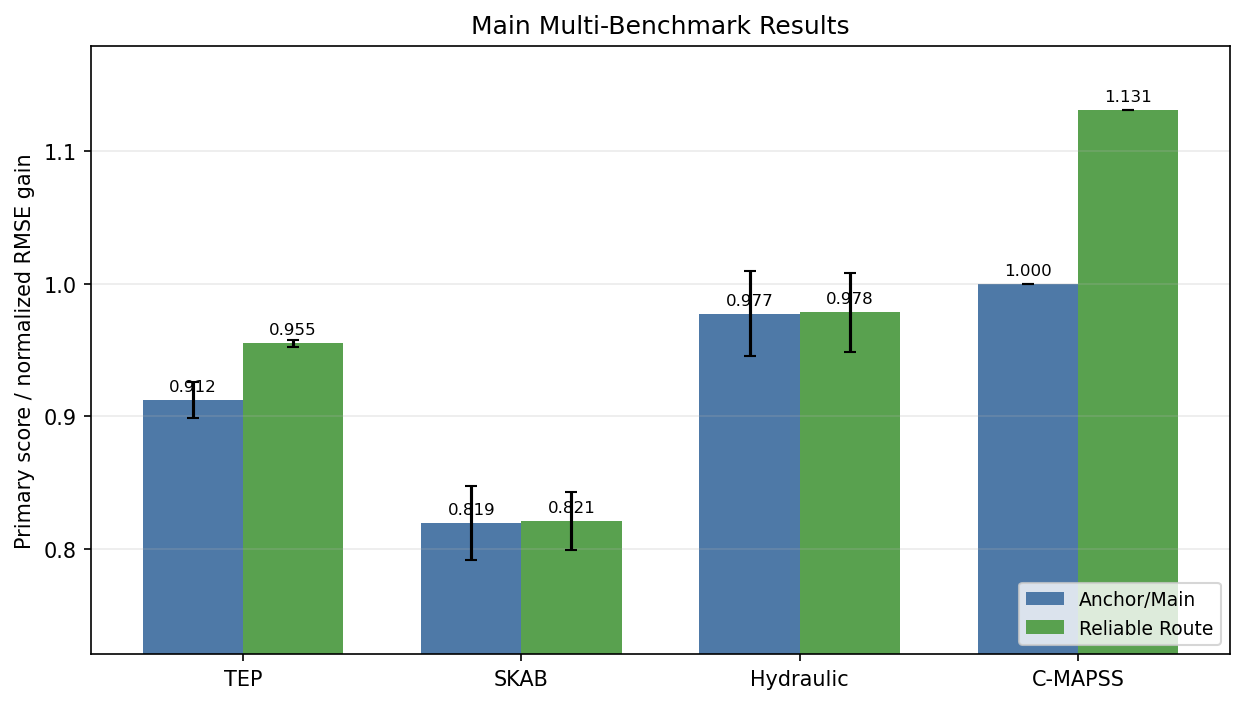
\includegraphics[width=0.98\textwidth]{figures/main_multi_benchmark_results.png}
  \caption{Main matched-protocol experiment results. C-MAPSS is normalized from RMSE because lower is better, while the dedicated RUL figure reports the original units.}
  \label{fig:main-experiment}
\end{figure*}

\subsection{Matched Backbone Controls}

To separate mechanism-evidence fusion from simply choosing a fashionable temporal backbone, we also ran local matched adapters for three strong external families: PatchTST, Anomaly Transformer, and Graph WaveNet. These are not official external scores because their native tasks are forecasting, anomaly scoring, or traffic forecasting rather than strict 22-class TEP diagnosis. Under the same TEP adapter protocol, the three-seed probes are much weaker than the reliability-calibrated mechanism route (Table~\ref{tab:backbone-controls}). We therefore use them as negative controls: they support the paper's claim that the main contribution is reliable admission of mechanism evidence, not direct transplantation of a generic backbone. We additionally archive official-source adapted budget probes for PatchTST, Anomaly Transformer, and Graph WaveNet. These runs fix source provenance but still add task-specific heads or protocol patches; PatchTST reaches only $0.4197 \pm 0.0320$ TEP Target-F1, Graph WaveNet reaches $0.2854 \pm 0.0529$, and Anomaly Transformer reaches $0.4716 \pm 0.0487$ SKAB Macro-F1 with 100\% FAR. They remain supporting negative controls rather than official external benchmark scores.

\begin{table}[t]
\centering
\caption{Official-source adapted matched controls. These rows fix source provenance but remain negative controls, not official external benchmark scores.}
\label{tab:backbone-controls}
\scriptsize
\setlength{\tabcolsep}{3pt}
\begin{tabular}{p{0.25\linewidth}p{0.23\linewidth}p{0.34\linewidth}}
\toprule
Backbone & Native family & Matched result \\
\midrule
PatchTST & patch Transformer forecasting & TEP Target-F1 $0.4197 \pm 0.0320$ \\
Graph WaveNet & adaptive graph-temporal forecasting & TEP Target-F1 $0.2854 \pm 0.0529$ \\
Anomaly Transformer & assoc.-discrepancy anomaly scoring & SKAB Macro-F1 $0.4716 \pm 0.0487$, FAR $100\%$ \\
\bottomrule
\end{tabular}
\end{table}

\subsection{Efficiency Audit}

We report efficiency only when the seed-level JSON artifact records parameter count, training time, and inference throughput. SKAB, C-MAPSS, and the TEP GDN/MTAD sequence baselines currently satisfy this requirement. For TEP, efficiency is measured from timed reruns, while the performance comparison preserves the best recovered target-F1 rows.

\begin{table*}[t]
\centering
\caption{Measured efficiency evidence. TEP sequence efficiency uses full-budget timed reruns; TEP performance comparisons keep the best recovered target-F1 rows.}
\label{tab:efficiency}
\small
\begin{tabular}{lrrr}
\toprule
Branch & Params & Train sec. & Test samples/s \\
\midrule
SKAB anchor & 88,716 & 340.54 & 2,988.7 \\
SKAB LLM verifier & 88,716 & 345.44 & 2,939.9 \\
C-MAPSS RUL anchor & 119,183 & 62.84 & 9,667.1 \\
C-MAPSS AnchorPath-BiGRU challenger & 382,162 & 147.46 & 8,341.6 \\
TEP GDN no/resid. & 17,942 / 35,885 & 0.47 / 0.63 & 586,309.7 / 330,096.4 \\
TEP MTAD no/resid. & 92,055 / 184,111 & 0.66 / 1.07 & 476,639.1 / 254,825.4 \\
\bottomrule
\end{tabular}
\end{table*}

\subsection{Ablations}

The ablation design separates three effects: the strength of the anchor, the benefit of mechanism challengers, and the reliability of admission. Removing reliability admission tests whether unfiltered expert or LLM-conditioned edges cause negative transfer. Removing LLM condition-verifier features tests whether semantic expert-edge activation helps difficult classes after validation. Removing lagged graph and residual channels tests whether temporal propagation evidence is necessary beyond static window features.

\begin{table}[t]
\centering
\caption{Ablation logic for internal mechanism validation.}
\label{tab:ablation}
\small
\begin{tabular}{p{0.30\linewidth}p{0.60\linewidth}}
\toprule
Variant & Purpose \\
\midrule
Anchor only & Tests base temporal discrimination \\
All evidence, no ERE & Tests unsafe knowledge injection \\
Expert only & Tests hand-written mechanism value \\
LLM only & Tests conditional expert-edge verification features \\
Lag/residual only & Tests temporal propagation evidence \\
Full model & Tests reliability-calibrated fusion \\
\bottomrule
\end{tabular}
\end{table}

\begin{figure*}[t]
  \centering
  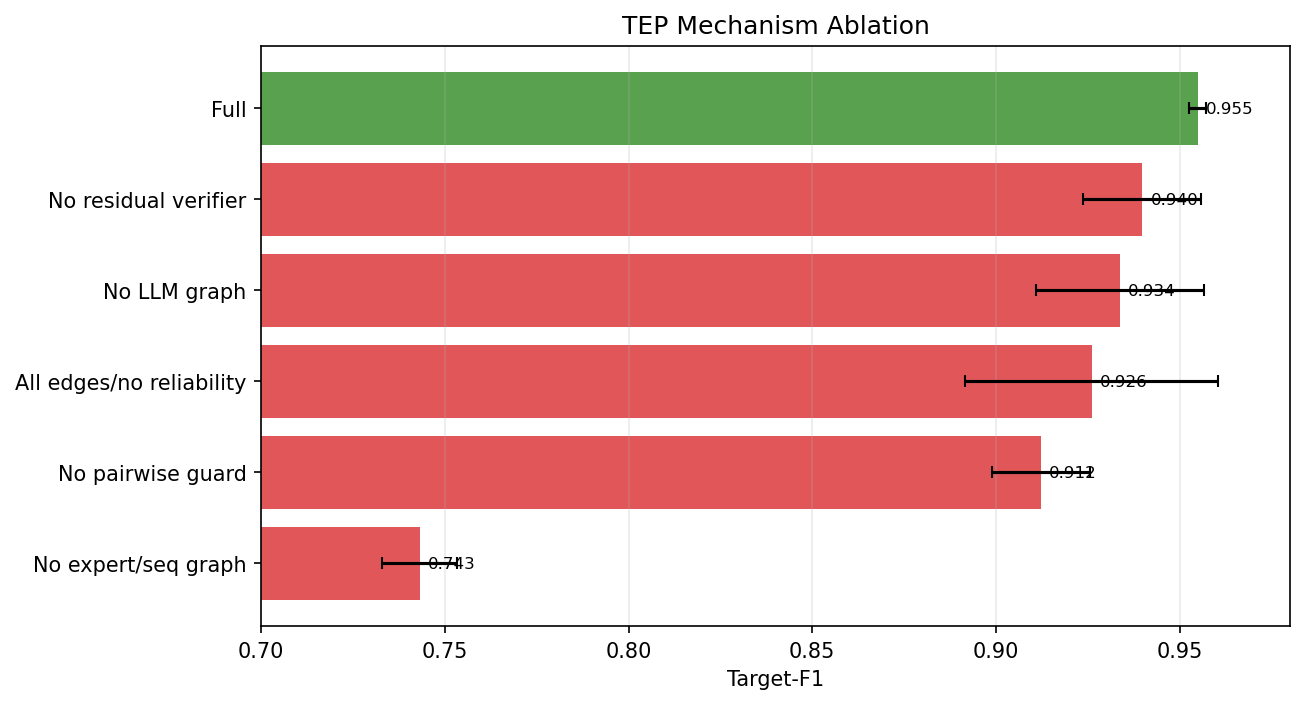
\includegraphics[width=0.98\textwidth]{figures/tep_mechanism_ablation.png}
  \caption{TEP mechanism ablation. The results show that improvement is not merely from adding more features, but from reliability-controlled mechanism admission.}
  \label{fig:ablation}
\end{figure*}

\subsection{Safety and Transfer}

Safety experiments evaluate whether the framework avoids damaging high-performing anchors and low-tail groups. Counterfactual edge perturbations test model dependence on admitted paths, while source and complexity penalties prevent dense LLM-generated graphs from overwhelming observed evidence. The expected outcome is not that every dataset reaches a universal leaderboard state-of-the-art score, but that admitted evidence improves the anchor when useful and falls back safely when unreliable.

\begin{figure*}[t]
  \centering
  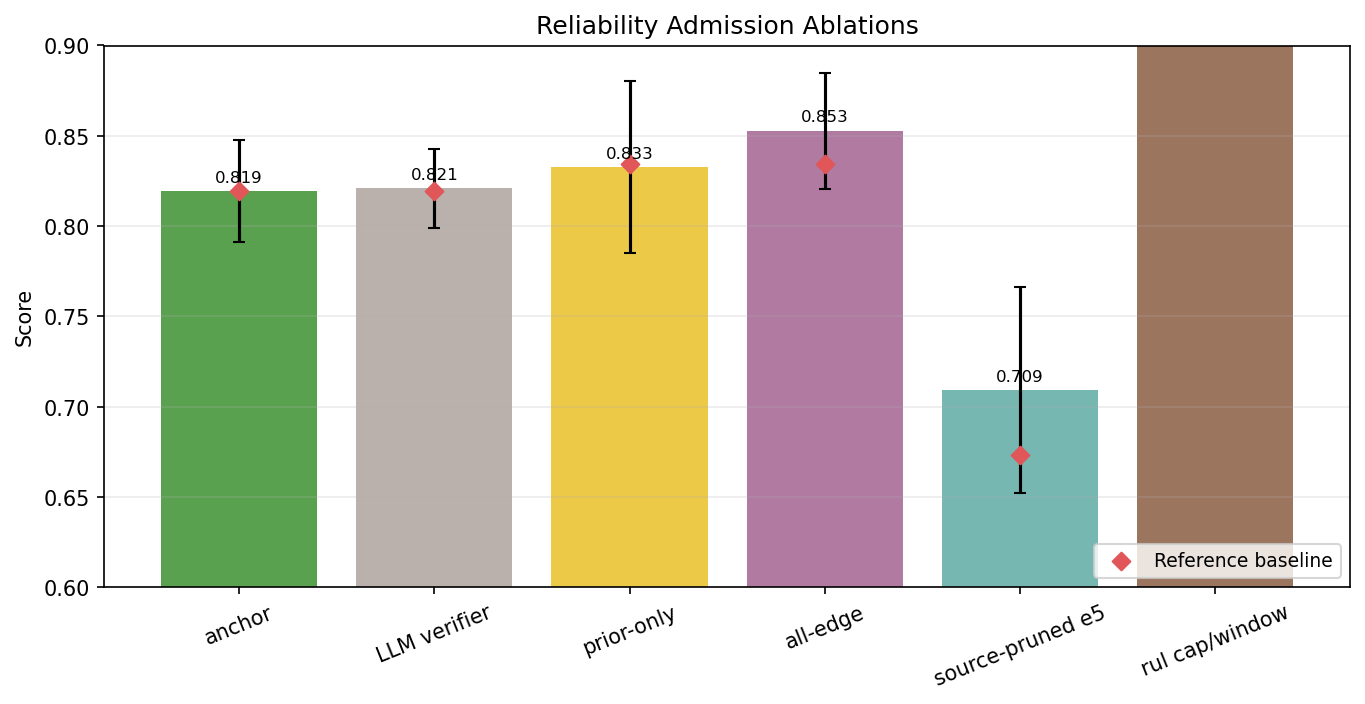
\includegraphics[width=0.98\textwidth]{figures/reliability_ablation_summary.png}
  \caption{Reliability ablation summary. The framework is evaluated by validation admission, unsafe prior-only/all-edge contrasts, source pruning, and original-task RUL transfer.}
  \label{fig:safety}
\end{figure*}

\begin{figure}[t]
  \centering
  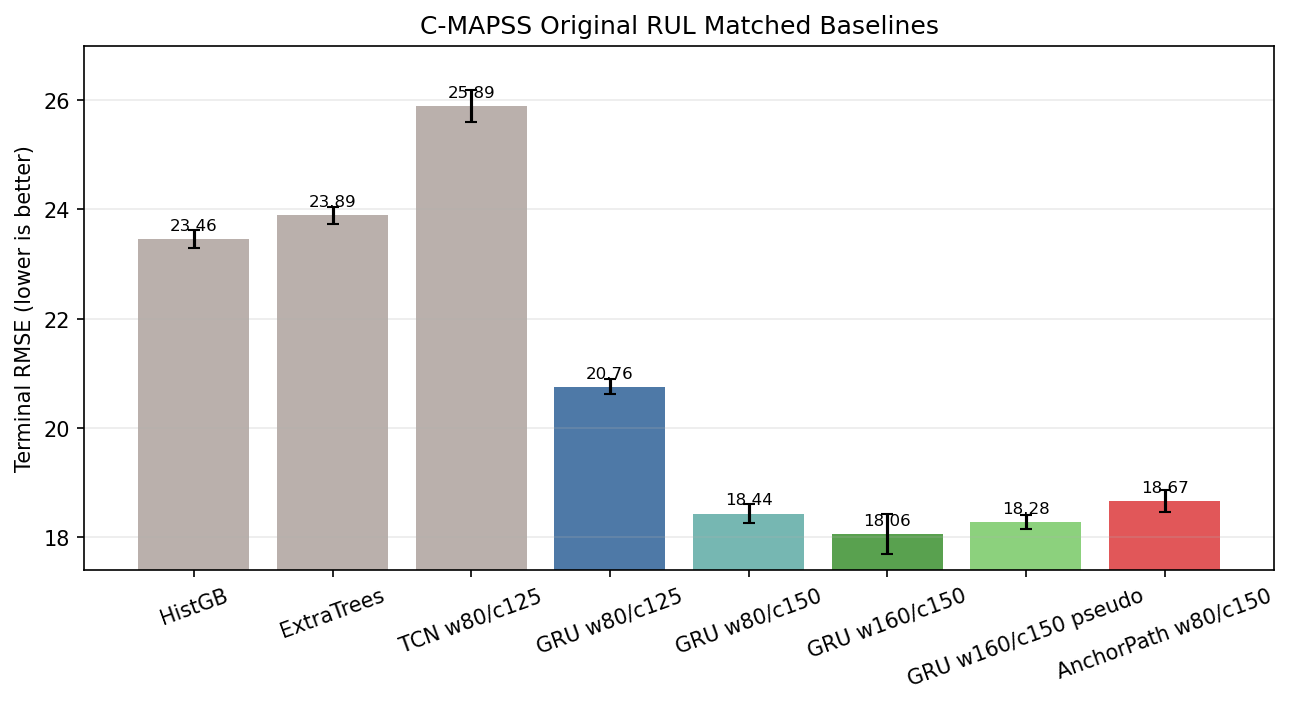
\includegraphics[width=0.98\linewidth]{figures/cmapss_rul_matched_results.png}
  \caption{C-MAPSS original terminal RUL regression. Lower RMSE is better; the current reliable branch is the cap-corrected long-window temporal anchor, and a train-unit pseudo-terminal audit selects the same configuration by RMSE while reporting a PHM-score trade-off. AnchorPath-BiGRU remains a non-admitted path-fusion challenger.}
  \label{fig:cmapss-rul}
\end{figure}

\section{Limitations}

The current framework provides reliability-calibrated evidence admission, not physical causal discovery. Counterfactual perturbation verifies model dependence on a proposed route; it does not replace plant-level intervention. The present evidence should be described as strong matched-protocol evidence until official benchmark protocols are exactly reproduced. The strongest current claim is mechanism-aware improvement and safe preservation across diverse industrial datasets, with TEP serving as the primary multi-class diagnosis setting.

\section{Conclusion}

We presented a reliability-calibrated framework for using imperfect mechanism evidence in industrial time-series fault diagnosis. The central idea is to keep a strong anchor predictor as the default and allow expert, LLM, lagged, residual, and graph evidence to correct it only when that evidence is validated, safe, and locally useful. This turns mechanism fusion from unchecked knowledge injection into a testable anchor-challenger admission problem, making the approach more suitable for non-interventional industrial settings where real causal verification is rarely available.

\bibliography{references}

\end{document}
